\documentclass[a4paper, onecolumn, 12pt]{article}
\usepackage[left=30mm,right=30mm,top=35mm,columnsep=15pt]{geometry} 
\usepackage[english]{babel} %language
\usepackage[utf8]{inputenc} %input encoding
\usepackage{float} %position of floating objects
\usepackage{bookmark} %hyperlinks in pdf
\usepackage{subcaption}
\usepackage[T1]{fontenc}
\usepackage{lipsum} %placeholder text
\usepackage{amsthm} %theorems
\usepackage{amsmath} %math
\usepackage{mathtools} %still math
\usepackage{listings} %code
\usepackage{xcolor} %syntax highlighting
\usepackage{algorithm}
\usepackage{algpseudocode}

% custom commands
\newcommand\tab[1][.3cm]{\hspace*{#1}}
\newcommand\tabeq[1][.5cm]{\hspace*{#1}}
\lstnewenvironment{myverbatim}[1][]{
  \lstset{
    basicstyle=\ttfamily,
    frame=tb,
    #1
  }
}{}

% \usepackage{physics}
% \usepackage{graphicx}
% \usepackage{adjustbox}
% \usepackage{placeins}
% \usepackage{csquotes}
% \usepackage{graphicx}
% \usepackage{tikz}
% \usepackage[normalem]{ulem}
% \useunder{\uline}{\ul}{}

\title{Long-Horizon Vehicle Motion Planning and Control Through Serially Cascaded Model Complexity}
\author{Flavio Maiorana \and Flavio Volpi \and Andrea Ferrari}
\date{\today}

\begin{document}

\maketitle
\begin{abstract}
    We propose the implementation and experimentation of a motion planning and
    control framework for autonomous vehicles based on nonlinear
    model-predictive control.The work is mainly based on \cite{paper}. The code
    is publicly available at
    \href{https://github.com/neverorfrog/vehicle-control}{this GitHub
    repository}. 
\end{abstract}

\newpage
\tableofcontents

\newpage
\section{Introduction}

Model predictive control (MPC for short) is a control technique which, in
closed-loop, computes the control inputs by means of an optimization algorithm,
which uses a \textbf{model} of the system and measurements to \textbf{predict}
future states and act accordingly by choosing the "best" control action. 

\begin{equation}
\begin{aligned}
    \min_{u_0,...,u_{N-1}}{J(x,u)} \\
    \text{ subject to }
        \quad x_{k+1} = f(x_k,u_k) \\
        \quad x_0 = x(t) \\
        \quad u_{min} \leq u_k \leq u_{max}
\end{aligned}
\end{equation}

We call $J(x)$ the \textbf{cost function} and $f(x,u)$ the \textbf{model}. The
critical part of MPC lies in the two last rows. The second-last expresses the
fact that, for every planning horizon, the current state is the initial state:
this is a subtle but important difference with respect to, for example,
trajectory optimization. The last row entails an equally important concept which
pertains specifically MPC, namely constraints. In the end, the sequence of
control actions is generated such that the cost function is minimized over the
\textbf{prediction horizon} by solving a constrained optimization problem that
depends on the evolution of the model over the horizon itself. Then, the
controller applies just the first action: in this way the system has advanced
one step, a new optimization problem with a new initial state is produced, and
the process goes on. The advantages of MPC are many: it is a multivaribale
controller, so it can control outputs by handling simultaneously all the
interactions between system variables; as said, it can handle constraints, so it
allows to avoid possible undesired states; it predicts the future states,
allowing to incorporate their information in the actual control. It is
particulary useful for a real-time control that adapts to \textbf{changes in the
environment}.\\
When dealing with nonlinear dynamics, a nonlinear MPC (or NMPC) can be used to
capture more accurately the nonlinear behavior of a system. This entails a more
robust manipulation capability of both nonlinearities and uncertainties in the
system. However, one of its major problems is the computational power it can
require, especially when dealing with highly nonlinear systems. This entails the
need of a high-performance hardware to solve the optimization problem in an
acceptable time, but sometimes this is not enough. Especially in a real
environment, where the timeliness is fundamental to take a decision,
computational efficiency is of utmost importance.\\
The purpose of \cite{paper} is to develop a novel, more computionally
cost-effective approach for a real-time NMPC for an autonomous vehicle, which
was tested in a race environment, where the objective was to complete a lap in
the minimum possible time, considering the actual capabilities of the vehicle.
The architecture consists in a so-called \textbf{cascaded model}, composed by a
detailed model of the car for the near term, and a simpler model used for
planning in the long term. This concept will be addressed more in detail.\\
In this work we tried to replicate the architecture of the paper from scratch,
testing the code in a very simple simulated race environment. Our purpose is to
show that, as claimed by \cite{paper}, the average computation time for the
cascaded model is lower, achieving also better results in terms of lap time.

\subsection*{Outline}

In the next section we will talk about some related work. After that, we will
address the modeling part of the algorithm in a rather formal way. Then, we will
formalize the NLP structure and put everything together to define the complete
MPC problem. Right after, we will discuss In the end, we will discuss some experiments and the results.

\section{Related Work}

\begin{itemize}
    \item Learning-based approach for vehicle control in \cite{rosolia}
    \item Linearization approach in \cite{bemporad}
\end{itemize}

\newpage
\section{Models}

Models must be well-defined to be used in NMPC. It is important to note that, as
said in \cite{paper}, the cascaded model together with the NLP formulation has
the precise goal to solve the problem of pushing a car to its physical
boundaries, like in race, while maintaining real-time performance. In this
section we will describe the main concepts behind the modeling part of the NMPC
algorithm. 

\subsection{Serially cascaded dynamical model}
Broadly speaking, while a single control loop system is a simple structure that
consists in just one primary loop that regulates directly the system, the
cascade control makes use of multiple control loops nested within each other.
The requirements for an effective cascade control are that the inner loops
variables must be faster-responding than the outer ones, and the major
disturbances enter in the inner loops. Considering the simplest cascade control
structure,\\
... (aggiungi schema/equazioni generiche del cascade semplice)

According to the control objectives, a cascade control scheme can include also 
more than one model in its control loops, such that each model capture different
relevant dynamics meeting different control tasks. In this way there is not the 
need to use a high-fidelity model for every objective, because some of them can 
be achieved considering simpler dynamic models. Furthermore, in optimal control
the usage of detailed models for long horizon can bring to an explosion of the 
complexity of the problem; instead, using more detailed models for near terms 
to have a high-fidelity of the real robot, and easier models for planning purpose
in long terms, allows to achieve good performances with computational limits.

When dealing with more than one dynamic model with different dynamic speeds,
the main advantage of a cascade control scheme is the higher performace with respect
to a simple single control loop, thanks to the possibility to control disturbances
in the inner loop before they affect the outer one. The main problem this architecture
can face is in the interaction between the control loops, where the reference signals 
generated by a control loop are not achievable by the others. This happens especially
when we are dealing with models with different complexity levels.

To deal with the disadvantages of the cascade control design, but leveraging on
its strengths, the idea of \cite{paper} in the scenario of an autonomous car is
to build a serial architecture which contains two dynamic models, belonging to
the same single control loop and the same prediction horizon. The first one is a
single-track vehicle model, which reflects comprehensively the complex dynamic
of the car (we will see in the next section the details) and provides all the
tools to accurately treat the first prediction steps. The farthest window of the
horizon is treated with a planar point-mass model, useful for long-term
trajectory planning with low computational resources. Thus the benefits of the
cascade model for the trajectory task are preserved; moreover the existance of a
single control loop ensure the feasibility of the reference targets that are
exchanged between the two models. A very important aspect to pay attention to
lies in the linkage of the plant models, namely propagating correctly the final
state of the first model to the initial state of the second model, and
mantaining consistency in constraints and cost functions across interconnected
models. 


\subsubsection{Single-track dynamic model}
The car can be represented as a dynamic bicycle model, where the two pairs of
front and rear wheels can be merged into a single wheel, one front wheel and one
rear wheel.\\
For the intrinsic properties, the vehicle is assumed to have a mass $\mathbf{m}$
and a yaw moment of inertia $\mathbf{I_{zz}}$; the wheelbase has length
$\mathbf{L}$, divided into $\mathbf{a}$ and $\mathbf{b}$, where they are
respectively the distances between the Center of Gravity and the front and rear
axle; the CG is at a distance $\mathbf{h_{cg}}$ from the ground; the front steer
angle is $\mathbf{\delta}$.\\
Since the model is of second-order, the state is composed of a velocity
component and a position/orientation one. The first one consists of the
longitudinal speed $\mathbf{U_x}$, the lateral speed $\mathbf{U_y}$, and the yaw
rate $\mathbf{r}$ of the CG. Meanwhile, the pose component is expressed in
relative coordinates withe respect to the road descriptor, namely by the
curvilinear coordinate $\mathbf{s}$, the lateral distance $\mathbf{e}$, and the
orientation of the chassis $\mathbf{\Delta \varPsi}$ with respect to the road
descriptor path. The curvature of the path, which is necessary to compute the
curvilinear coordinate and the orientation is called $\mathbf{\kappa}$. Thus, we
can at every time instant identify a unique pose of the vehicle by the tuple
$s,e,\Delta \varPsi$, as already said in section \ref*{subsec:track}.\\
The inputs of the system are the steering angle rate $\dot{\delta}$ and the
total longitudinal force $F_x$. This one can be divided in the longitudinal
force applied on the axle of the front tire $F_{x_f}$ and the longitudinal force
applied on the axle of the rear tire $F_{x_r}$, according to a distribution
function $\tilde{\chi}$:
\begin{subequations}
    \begin{eqnarray}
        \tilde{\chi_f} &=& \frac{d_f - b_f}{2}\tanh(2(F_x+0.5))+\frac{d_f+b_f}{2} \\
        \tilde{\chi_r} &=& \frac{b_r-d_r}{2}\tanh(-2(F_x+0.5))+\frac{d_r+b_r}{2}
    \end{eqnarray}
\end{subequations}
where $d_f$ and $d_r$ represent the drive force distribution, and $b_f$ and $b_r$ represent the 
brake force distribution. So the single components of the longitudinal force are:
\begin{subequations}
    \begin{eqnarray}
        \tilde{F}_{x_f} &=& \tilde{\chi}_f(F_x) \cdot F_x \\
        \tilde{F}_{x_r} &=& \tilde{\chi}_r(F_x) \cdot F_x
    \end{eqnarray}
\end{subequations}
This implementation might seem rather complex, compared to simply expressing the front and rear force distribution as
\begin{subequations}
    \begin{eqnarray}
        \tilde{F}_{x_f} = \tilde{\chi}_f \cdot F_x \\
        \tilde{F}_{x_r} = \tilde{\chi}_r \cdot F_x
    \end{eqnarray}
\end{subequations}
where $\tilde{\chi}_f$ and $\tilde{\chi}_r$ are scalars that sum to 1, however, these equations will be used for numerical 
optimization, and should therefore be twice differentiable, and we therefore have to use the workaround equations presented above. \\
For the tire model, given the maximum instantaneous normal load of the tire $F_z$, the maximum possible
lateral tire force that can be obtained applying the input force $\tilde{F}_x$ is:
\begin{equation}
    \tilde{F}_y^{max} = \sqrt[]{(\mu F_z)^2 - (0.99\cdot \tilde{F}_x)^2}
\end{equation}
where $\mu$ is the tire-road friction coefficient and the 99\%  of the longitudinal force is due to solve 
some numerical issues in the optimization problem. \\
The normal loads for the two tires are affected also by the slope $\theta$ of the road, and by the banking $\phi$, in the following way:
\begin{subequations}
    \begin{eqnarray}
        \label{normal}
        F_{z_f} = \frac{b}{L}m(g\cdot \cos(\theta)\cos(\varphi)+A_{V^2}U_x^2)-\frac{h_{cg}}{L}F_x \\
        F_{z_r} = \frac{a}{L}m(g\cdot \cos(\theta)\cos(\varphi)+A_{V^2}U_x^2)+\frac{h_{cg}}{L}F_x
    \end{eqnarray}
\end{subequations}
where the effect of vertical curvature on speed are expressed through:
\begin{equation}
    A_{V^2} = -\frac{\partial \theta}{\partial s}\cos(\varphi)-\kappa\cdot \sin(\varphi)\cos(\theta) 
\end{equation}
The slip angles of the front ($\alpha_f$) and rear ($\alpha_r$) wheels are respectively given by:
\begin{subequations}
    \begin{eqnarray}
        \alpha_f &=& \arctan \left(\frac{U_y+ar}{U_x}\right)-\delta \\
        \alpha_r &=& \arctan \left(\frac{U_y-br}{U_x}\right)
    \end{eqnarray}
\end{subequations}
A full sliding occurs at an angle denoted as $\alpha^{\text{mod}}$, which is calculated as:
\begin{equation}
    \alpha^{\text{mod}} = \arctan\left(\frac{3\cdot F_y^{\text{max}}\cdot\zeta}{C_{\alpha}}\right)
\end{equation}
Here, $\zeta$ is a factor introduced to ensure the tire model's strict monotonicity.\\
Thus, considering $\alpha = \left(\alpha_f \tab \alpha_r\right)^T$, the tire model can
be expressed as:
\begin{equation}
    F_y = 
    \left\{
	\begin{array}{ll}
		-C_\alpha \tan(\alpha)+&\\
        \tabeq\frac{C_\alpha^2}{3\tilde{F}_y^{max}}|\tan(\alpha)|\tan(\alpha) - &\\
        \tabeq\frac{C_\alpha^3}{27(\tilde{F}_{y}^{max})^2}\tan^3(\alpha) 
        & \mbox{if } |\alpha| \leq \alpha^{mod} \\
		-C_{\alpha}(1-2\zeta+\zeta^2)\tan(\alpha)-&\\
        \tabeq \tilde{F}_y^{max}(3\zeta^2-2\zeta^3){sgn(\alpha)}
        & \mbox{otherwise }
	\end{array}
    \right.
\end{equation}
\\
Regarding the drag forces, these are included all in the same variable $F_d$:
\begin{equation}
    \label{drag_force}
    F_d = F_{rr}+C_DU_x^2-mg\sin(\theta)
\end{equation}
where $F_{rr}$ represents the rolling resistance, $C_D$ is the coefficient of aerodynamic
drag. \\
Instead, the lateral force $F_b$ applied on the CG models the effect of the road bank angle $\varphi$:
\begin{equation}
    \label{lateral_force}
    F_b = -mg\cos(\theta)\sin(\varphi)
\end{equation}
\\
\\
All these informations are used to describe the motion of the single-track model:
\begin{subequations}
    \begin{eqnarray} 
        \dot{U}_x &=& \frac{\tilde{F}_{x_f}\cos(\delta)-\tilde{F}_{y_f}\sin(\delta)+\tilde{F}_{x_r}-F_d}{m}+rU_y\\
        \dot{U_y} &=& \frac{\tilde{F}_{y_f}\cos(\delta)+\tilde{F}_{x_f}\sin(\delta)+\tilde{F}_{y_r}+F_b}{m}-rU_x\\ 
        \dot{r} &=& \frac{a(\tilde{F}_{y_f}\cos(\delta)+\tilde{F}_{x_f}\sin(\delta))-b\tilde{F}_{y_r}}{I_{zz}}\\
        \dot{s} &=& \frac{U_x\cos(\Delta \varPsi) -U_y\sin(\Delta \varPsi)}{1-\kappa e}\\
        \dot{e} &=& U_x\sin(\Delta \varPsi)+U_y \cos(\Delta \varPsi)\\
        \Delta \dot{\varPsi} &=& r-\kappa \dot{s}
    \end{eqnarray}
\end{subequations}

\subsubsection{Point-Mass model}
The Point-Mass model is a simpler version of the Single-Track model, where the car is approximated with a point object
in the Center of Gravity of the vehicle. Being a one-dimensional object, the point has just one total horizontal velocity state $\bar{V}$, 
and three position states relative to the road descriptor path: the distance $\bar{s}$ along it, the lateral distance $\bar{e}$ from it, and finally the
difference in orientation $\bar{\phi}$ between the velocity vector and the tangent to the road descriptor path.

Substituting ${U}_x$ with $\bar{V}$, we can use some of the equations introduced in the single-track model also for the point-mass model,
in particular for the drag force ${F}_d$ (eq. \ref{drag_force}), for ${F}_b$ (eq. \ref{lateral_force}) and for the normal loads ${F}_{z_f}$ and ${F}_{z_r}$ (eq. \ref{normal}).
Following the basic intuition of having to simplify the model, the tire forces are not modeled.

The inputs to this model are the longitudinal force $\bar{F}_x$ and the lateral force $\bar{F}_y$, that are limited by friction limits
according to the following rules:
\begin{subequations}
    \begin{eqnarray} 
        \left(\frac{b}{L}\bar{F}_y\right)^2 + \left(\tilde{\chi_f}\bar{F}_x\right)^2 \leq \left(\mu_f F_{z_f}\right)^2 \\
        \left(\frac{a}{L}\bar{F}_y\right)^2 + \left(\tilde{\chi_r}\bar{F}_x\right)^2 \leq \left(\mu_r F_{z_r}\right)^2
    \end{eqnarray}
\end{subequations}
Thus the equations that describe the motion of the point-mass model are the following:
\begin{subequations}
    \begin{eqnarray}
        \dot{\bar{V}} &=& \frac{\bar{F}_{x}-\bar{F}_{d}}{m}\\
        \dot{\bar{s}} &=& \frac{\bar{V}\cos(\bar{\phi})}{1-\kappa \bar{e}}\\
        \dot{\bar{e}} &=& \bar{V}\sin(\bar{\phi})\\
        \dot{\bar{\phi}} &=& \frac{{\bar{F}}_y + {\bar{F}}_b}{m\bar{V}} - k\dot{\bar{s}}
    \end{eqnarray}
\end{subequations}

Note that the yaw dynamics are omitted, and therefore this model cannot be used for yaw stabilization

\subsubsection{Propagating the state from single-track to point-mass}
Here we define the mapping from the single-track to the point-mass states. 
It is very important that this mapping is correct, to guarantee that the transition
from one model to the other is compliant to the reality.\\
The mapping, called $spatialTransition_{trans}(x_k)$, is the following:
\begin{subequations}
    \begin{eqnarray}
        \bar{V} &=& \sqrt{U_{x}^{2}-U_{y}^{2}}\\
        \bar{s} &=& s\\
        \bar{e} &=& e\\
        \bar{\phi} &=& arctan\left(\frac{{U}_y}{{U}_x}\right) + \Delta\psi
    \end{eqnarray}
\end{subequations}

\subsection{Spatial dynamics} \label{spatial}
Since the dynamical models need to be used in a digital fashion, it has to be
discretized. The discretization of the models can be done with respect to time
or with respect to space, according to own purposes, with the respective pros
and cons.
\begin{description}
    \item[Discretizing in time] consists in dividing the time over the horizon in
    small well-defined time intervals $dt$, and leaving the spatial curvilinear
    coordinate $s$ as an optimization variable in the NLP. This approach implies
    that we know beforehand the temporal window for the horizon. Since this is
    the most straightforward wa to discretize, it is also more intuitive.
    Nevertheless, there are some problems attached to it, especially in a car
    racing scenario. Since the curvilinear abscissa acts as a variable, it
    cannot be keep fixed inside of a single time interval, which means that the
    path geometry will be obtained by some interpolation function to be
    evaluated during the planning horizon. This can cause some issues,
    computation-wise.
    \item[Discretizing in space] means to establish the spatial
    discretization steps $ds$ that compose the total space travelled by the
    vehicle in the horizon window. In this way the time $t$ can be left as an
    optimization variable. In contrast, this method does not allow to the car to
    stop, but this is not a problem for our purposes. Instead, a good advantage
    of the spatial discretization is that during each \textbf{space interval},
    the path geometry is known and constant, and thus can be computed apriori,
    before even starting the planning horizon. Moreover, space discretization
    allows to easily add elements to the track which are always know apriori,
    like static obstacles, without creating too much trouble.
\end{description}
For the reasons stated above, since we are a racing scenario in which time
minimization is of paramount importance, and the track geometry is known
apriori, the spatial discretization method is the more adequate for the MPC
planning horizon. This means that outside the horizon, the dynamical model will
evolve as usual, following a time-discretized differential equation, while
inside the MPC the evolution is space-disretized. Thus, denoting as $p$ a state
variable of any model, we define its derivative with respect to the curvilinear
coordinate $s$ as
\begin{equation}
    p' = \frac{d p}{d s} = \frac{dp}{dt} \frac{dt}{ds} = \dot{p} \frac{dt}{ds} = \dot{p} \frac{1}{\dot{s}}
\end{equation}  
that we will compute through the chain rule.
According to this notation, we can define the spatial dynamics for the single-track model as such:
\begin{subequations}
    \begin{eqnarray}
        U'_x &=& \left(\frac{\tilde{F}_{x_f}\cos(\delta)-\tilde{F}_{y_f}\sin(\delta)+\tilde{F}_{x_r}-F_d}{m}+rU_y\right) \frac{1}{\dot{s}}\\
        U'_y &=& \left(\frac{\tilde{F}_{y_f}\cos(\delta)+\tilde{F}_{x_f}\sin(\delta)+\tilde{F}_{y_r}+F_b}{m}-rU_x\right) \frac{1}{\dot{s}}\\
        r' &=& \left(\frac{a(\tilde{F}_{y_f}\cos(\delta)+\tilde{F}_{x_f}\sin(\delta))-b\tilde{F}_{y_r}}{I_{zz}}\right) \frac{1}{\dot{s}}\\
        e' &=& \left(U_x\sin(\Delta \varPsi)+U_y \cos(\Delta \varPsi)\right) \frac{1}{\dot{s}}\\
        \Delta \varPsi' &=& \left(r-\kappa \dot{s}\right) \frac{1}{\dot{s}}\\
        \delta ' &=& \frac{\dot{\delta}}{\dot{s}}\\
        t' &=& \frac{1}{\dot{s}}
    \end{eqnarray}
\end{subequations}
and for the point-mass model:
\begin{subequations}
    \begin{eqnarray}
        {\bar{V}}' &=& \left(\frac{\bar{F}_{x}-\bar{F}_{d}}{m}\right) \frac{1}{\dot{\bar{s}}}\\
        {\bar{e}}' &=& \left(\bar{V}\sin(\bar{\phi})\right)\frac{1}{\dot{\bar{s}}}\\
        {\bar{\phi}}' &=& \left(\frac{{\bar{F}}_y + {\bar{F}}_b}{m\bar{V}} - k\dot{\bar{s}}\right)\frac{1}{\dot{\bar{s}}}\\
        \bar{t}' &=& \frac{1}{\dot{\bar{s}}}
    \end{eqnarray}
\end{subequations}
We will denote in a concise way the spatial transitions from a state to the next one as
$spatialTransition_{st}(x_k, u_k)$ for the single-track, and $spatialTransition_{pm}(x_k, u_k)$ 
for the point-mass model, where $x_k$ is the state at time step $k$ and $u_k$ is the control
applied at time step $k$. 


\newpage
\section{NLP Structure}

The key element of the NLP is the cost function, which can be composed by many terms according to own purposes.
Our objective is to minimize time along the finite planning horizon, while also respecting the road
boundaries and while keeping the car in a safe configuration. 
To achieve this, a series of terms regarding both single-track and point-mass models are summed together:
\begin{enumerate}
    \item \textbf{Final time}: the time $\bar{\tau}_M$ at which the point-mass model reaches the last stage of the planning horizon
    \item \textbf{Terminal state}: to make sure that the final stage is a safe one, we add this penalty based on the 
    lateral position ${\bar{e}}_m$, the course error ${\bar{\phi}}_m$ and the excess speed ${\bar{V}}_{exc}$ of the final stage, with
    \begin{equation}
    {\bar{V}}_{exc} = 
    \left\{
	\begin{array}{ll}
		{\bar{V}}_m - {{\bar{V}}_{safe}}
        & \mbox{if } {\bar{V}}_m > {{\bar{V}}_{safe}} \\
	0 & \mbox{otherwise }
	\end{array}
    \right.
    \end{equation}

    The terms introduced are finally combined in
    
    \begin{equation}{J}_{term} = W_{e_{term}}{\bar{e}}_m^2 + {W_{\phi}}_{term}{\bar{\phi}}_m^2 + {W_V}_{term}{\bar{V}}_{exc}^2
    \end{equation}

    \item \textbf{Road Boundary Intrusion}: it penalizes when the car crosses the track boundaries
    \begin{equation}
    J_{rb} = W_{rb}\sum_{k=1}^{N} \Delta s_k \begin{cases}
    (e_k - {e_{\text{max}}}_k)^2, & \text{if } e_k \geq e_{\text{max}_k} \\
    (e_k - e_{\text{min}_k})^2, & \text{if } e_k \leq e_{\text{min}_k} \\
    0, & \text{otherwise}
    \end{cases}
    \end{equation}
    \[  + W_{rb}\sum_{l=1}^{M} \Delta\overline{s}_l \begin{cases}
    (\overline{e}_l - \overline{e}_{\text{max}_l})^2, & \text{if } \overline{e}_l \geq \overline{e}_{\text{max}_l} \\
    (\overline{e}_l - \overline{e}_{\text{min}_l})^2, & \text{if } \overline{e}_l \leq \overline{e}_{\text{min}_l} \\
    0, & \text{otherwise}
    \end{cases}
    \]

    where, intuitively, ${e_{\text{max}}}_k$ can be chosen a little bit smaller than the width of the road.

    \item \textbf{Deviation from the Road Descriptor Path}: it encourages the car to stay as near as possible to the road descriptor
    \begin{equation}
    J_{rd} = W_{rd} \left( \sum_{k=1}^{N} \Delta s_k e_k^2 + \sum_{l=1}^{M} \Delta\overline{s}_l \overline{e}_l^2 \right)
    \end{equation}

    \item \textbf{Obstacles avoidance}: it discourages the car to go through the obstacles
    \begin{equation}
        J_{obs} = W_{obs} \left( \sum_{k=1}^{N} \sum_{j=1}^{J} \frac{\Delta s_k}{d_{j,k} - r_j} \right)
    \end{equation}
    where $k$ is the usual index counting the steps of the prediction horizon
    and $j$ is the index counting the obstacles on the track. Furthermore,
    \[d_{j,k} = \sqrt{(s_k-s_j)^2 + (e_k-e_j)^2}\] is the distance between the
    $k_{th}$ predicted car position and the $j_{th}$ obstacle, while $r_j$ is
    the radius of the $j_{th}$ obstacle.

    \item \textbf{Slew rate}: in order to encourage smooth controls we penalize too big increases of the steering rate $\dot{\delta}$, variation of the total lateral force $\Delta F_y$, variation of the new commanded longitudinal force ${F_x}_k$ with respect to the previous commanded ${F_x}_{k-1}$.
    And finally, the variation in forces at the model transition, denoted as $\Delta F_u$.
    These are all combined into:
    
    \begin{equation}
        J_{\dot{u}} = J_{\dot{\delta}} + J_{\Delta F_y} + J_{\Delta F_x} + J_{\Delta F_u}
    \end{equation}

    !!!To be completed, vogliamo esprimere le varie J di questo ultimo step o diventa troppo listone di equazioni?!!!
    
    \item \textbf{Excessive Slip Angle}: in order to discourage the car to operate in the fully saturated region of the tires, we add a penalty on excessive slip angle. This helps in stabilizing the car.
    \begin{equation}
        J_{a} = W_{a}\sum_{k=1}^{N}
        \begin{cases}
        \left(|\tan \alpha_{f_k}|-\tan \alpha_{f_k}^{\text{mod}}\right)^2, & \text{if } |\tan \alpha_{f_k}| \geq  \tan \alpha_{f_k}^{\text{mod}}\\
        0, & \text{otherwise}
        \end{cases}
        \end{equation}
        \[  + W_{a}\sum_{l=1}^{M} 
        \begin{cases}
        \left(|\tan \alpha_{r_k}|-\tan \alpha_{r_k}^{\text{mod}}\right)^2, & \text{if } |\tan \alpha_{r_k}| \geq  \tan \alpha_{r_k}^{\text{mod}}\\
        0, & \text{otherwise}
        \end{cases}
        \]
\end{enumerate}

The constraints of the NLP concern some limitations on the states of the single-track and of the point-mass models, 
on the input variables, on the tire model, and on the dynamics of the systems, including the transition between
them. In detail:
\begin{enumerate}
    \item \textbf{State limits}: the velocities $U_x$ and $\bar{V}$ are maintained greater than a minimum value, such 
    that they will never go to zero and the car will never stop. This is possible because we are in a race scenario.
    In this way some problems with spatial discretization and singularities in the models are avoided.\\
    Moreover, there are some mechanical limits on the steering angle $\delta$.
    \begin{align}
        U_{x_k} \geq U_x^{min} && \forall k=1,...,N\\
        \bar{V_l} \geq \bar{V^{min}} && \forall l=1,...,M\\
        \delta^{min} \leq \delta_k \leq \delta^{max} && \forall k=1,...,N
    \end{align}

    \item \textbf{Input limits}: the input longitudinal forces for both dynamic models have an upper bound, depending
    on the maximum engine power $P_{eng}$ and the longitudinal velocity; furthermore there is a range of possible values
    for the steering rate.
    \begin{align}
        F_{x_k} \leq \frac{P_{eng}}{U_{x_k}} && \forall k=0,...,N \\
        \bar{F}_{x_k} \leq \frac{P_{eng}}{\bar{V}_{x_l}} && \forall l=0,...,M \\
        \dot{\delta}^{min} \leq \dot{\delta}_{k} \leq \dot{\delta}^{max} && \forall k=0,...,N
    \end{align}

    \item \textbf{Tire model}: in the single-track model, the longitudinal tire forces are bounded by the friction forces 
    modified by the slip angle $\alpha$
    \begin{align}
        -\mu_f F_{z_{f_k}} \cos(\alpha_{f_k}) \leq \tilde{F}_{x_{f_k}} \leq \mu_f F_{z_{f_k}} \cos(\alpha_{f_k}) && \forall k=0,...,N \\
        -\mu_r F_{z_{r_k}} \cos(\alpha_{r_k}) \leq \tilde{F}_{x_{r_k}} \leq \mu_f F_{z_{r_k}} \cos(\alpha_{r_k}) && \forall k=0,...,N 
    \end{align}

    \item \textbf{Dynamics}: given a certain initial state for the single-track, the next states of this model must respect the
    spatial dynamics of the system explained in \ref{spatial}. Defined the vehicle state as $x$:
    \begin{eqnarray}
        x_0 &=& x_{\text{measured}} \\
        x_{k+1} &=& \text{spatialTransition}_{st}(x_k, u_k) \\
        \bar{x}_0 &=& \text{spatialTransition}_{trans}(x_N) \label{transition}\\
        \bar{x}_{k+1} &=& \text{spatialTransition}_{pm}(\bar{x}_k, \bar{u}_k)
    \end{eqnarray}
    where $x_{\text{measured}}$ is the current measured state and it must be the initial state of the single-track model,
    while the eq.\ref{transition} establishes that the initial state of the point-mass model comes from the propagation of 
    the last state of the single-track.
\end{enumerate}
As we can notice, the restriction to stay inside the track boundaries is modeled
not as a constraint, but like a cost term that increases when the car is outside
the nearest border, otherwise it is null. Similary, the collision with obstacles
is discouraged by minimizing the inverse of the distance to each obstacle, thus
penalizing small distances. Giving both terms high weights, we can be sure to
obtain a good result without imposing them as hard constraints. This approach is
prefered to the other one because it allows the NLP to be always numerically
feasible.

\newpage

\section{Implementation}

We used as main backbone CasADI (\cite{casadi}), a software framework for automatic
differentiation, nonlinear optimization and optimal control. It is implemented
in C++ and has also a python interface. Casadi serves three main purposes:
\begin{itemize}
    \item Modeling
    \item Simulation through numerical integration
    \item Formulation and solving of optimization problems within MPC
\end{itemize}
The "sofware framework" is based mainly on three components
\begin{description}
    \item[Controller] expressed as a CasADI nlp, namely a non-linear cost
    function with non-linear constraints, that spits out a single control action
    based on the current state and the predicted state for the next H steps (H
    is the horizon length)
    \item[Model] of the car, expressed as a casadi function that evolves the
    state of the dynamical model with respect to the current state and action
    \item[Simulator] to show everything graphically in real-time
\end{description}

\subsection{Simulator}

To simulate a real racing track and a car interacting with it, we just used
some simple plotting tools together with the modeling and numerical integration
capabilities of CasADI. The main goals of the simulator are:
\begin{itemize}
    \item Visualize the track with the car correctly localized depending on its state
    \item Simulate the car's movement
\end{itemize}
The complete implementation of the simulator can be found at
\href{https://github.com/neverorfrog/vehicle-control/blob/main/simulation/racing.py}{racing.py}.
Overall, the simulation loop can be summarized in pseudocode as follows.

\begin{algorithm}
    \caption{Simulation Loop}\label{sim}
    \begin{algorithmic}[1]
        \State $dt \gets 0.06$ s \Comment{Time step}
        \While{ one full turn not completed }
        \State measure car state $x$
        \State action $a \gets command(x)$ \Comment{From MPC}
        \State move forward for $dt$ under $a$ 
        \EndWhile
    \end{algorithmic}
\end{algorithm}

Line 3 takes the assumption that the state is fully known at each instant. We
take this assumption for simplifying reasons. In a real setting the state would
be measured with sensors and filtering algorithms. 

\newpage
\subsubsection*{Track}
\label{subsec:track}

Since the algorithm is application-specific for the race environment, it is
fundamental to model and represent the racing track itself. We decided to model
it as a sequence of \textbf{waypoints}, defining the track centerline, which are
then connected through a \textbf{cubic spline}. The waypoints are constructed
based on three user-defined parameters:
\begin{itemize}
    \item corner coordinates (in meters)
    \item resolution (meters between two waypoints)
    \item smoothing (number of waypoints considered for smoothing)
\end{itemize}
This way, we can \textbf{uniquely identify a pose} in the track through the
coordinates $\mathbf{s,e,\phi}$, namely the curvilinear abscissa, the position
error and the orientation error. We recall that they describe respectively the
displacement of the car along the track, the lateral error with respect to the
centerline and the yaw error with respect to the track orientation. As already
seen, the state of the car is expressed through these "relative" coordinates.
Similarly, obstacles are modeled by their relative coordinates $s,e$ and the
radius (in meters) $r$ (as a simplifying assumption, the obstacles are all
circular).

\begin{myverbatim}[title={Example of a track configuration file}]
corners: #[x, y]
    - [0, 0]
    - [60, 0]
    - [60, 60]
    - [-60, 60]
    - [-60, 0]
    - [0, 0]
resolution: 0.1 [m]
smoothing: 300 
width: 9 [m]
obstacle_data: #[s, ey, r]
    - [60, 2, 3]
    - [90,  3, 2]
    - [90, -3, 2]
    - [140, -2, 2]
    - [170, 2, 2]
    - [220, 0, 2]
\end{myverbatim}
\newpage 
The result would then be the one shown in figure \ref{ippodromo} below. The
track is pretty simple for testing purposes, but it is possible with much ease
to create more complex tracks, thanks to the flexibility of the waypoint
definition schema. \\
The main features of interest of the track are the following:
\begin{itemize}
    \item centerline position
    \item track curvature
    \item track orientation
\end{itemize}
\begin{figure}[h]
    \centering
    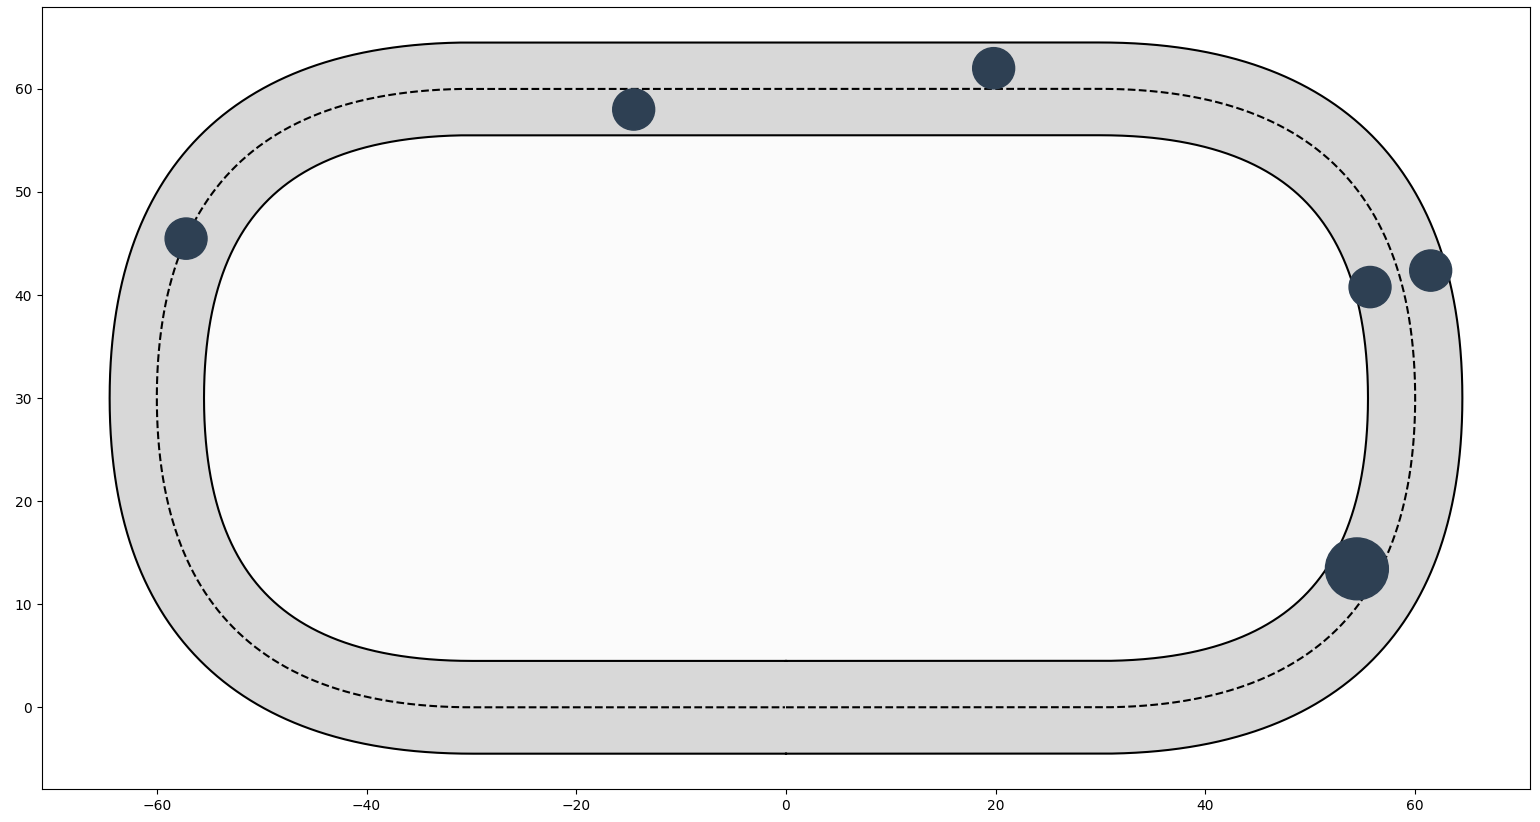
\includegraphics[width=\textwidth]{assets/ippodromo_obstacles.png}
    \caption{Example track with round obstacles}
    \label{ippodromo}
\end{figure} \vspace{0.5cm}
As for the centerline, we simply evaluate the spline defined through the
waypoints at the curvilinear abscissa $s$. We will define the two spline
functions, one for $x$ and one for $y$ as $x_{spline}(s)$ and $y_{spline}(s)$.\\
The curvature is defined as the inverse of the curvature radius and can be
expressed as
\begin{equation}
    \kappa(s) = \frac{x' \cdot y'' - y' \cdot x''}{\sqrt{(x'^2 + y'^2)^3}}
\end{equation}
where $x'$ and $y'$ are the derivatives of the absolute coordinates with respect
to the curvilinear abscissa $s$. We omitted the dependancy to $s$ in the
righthand-side of the above equation just for notation. The curvature
information is of utmost importance for the controller, since the evolution of
the relative coordinates depends on it. \\
Similarly, the orientation can be expressed as
\begin{equation}
    \phi(s) = \arctan\left(\frac{y'}{x'}\right)
\end{equation}
These two quantities are also needed to convert the relative coordinates to a
global coordinate system. We can express this change of coordinates as such:
\begin{equation}
    \Bigg\{
        \begin{array}{ll}
            x(s,e) =  x_{spline}(s) - sin(\phi(s)) \cdot e\\
            y(s,e) =  y_{spline}(s) + cos(\phi(s)) \cdot e\\
            \varPsi(s,\varPsi) = \phi(s) + \Delta \varPsi
        \end{array}
\end{equation}
This way, it is always possible to identify a pose in the track in global
coordinates, in order to plot the car. More information about the implementation
can be found in
\href{https://github.com/neverorfrog/vehicle-control/blob/main/environment/track.py}{track.py}


\subsection{Discretized model}

An important aspect, which was not mentioned when we treated the models in a
more formal way, is how the models are actually discretized. Conceptually, the
model is still expressed as a symbolic function through CasADI, as if it were a
continuous function, so nothing fancy about that. The discretization consists in
adding to the symbolic function an integrator, which has the scope of letting
the system transition from one state by applying a certain input, holding it for
a certain amount of time and integrating the state rate of change, to finally
end up into another state. In the pseudocode, it is line 5 we are talking about.
Practically speaking, what happens is that we create a \textit{discrete ode} in
form of a casadi function by executing the following steps:
\begin{enumerate}
    \item Define the righthand side of the continuous ode as a \textit{symbolic}
    casadi function, namely \[f(state,action,\kappa)\] In our case, taking just
    the singletrack model as an example, the state is the tuple
    \([U_x,U_y,r,\delta,s,e,\Delta\varPsi,t]\) and the action \([F_x,\omega]\).
    Instead, $\kappa$ indicates the curvature of the track. This function
    returns the rate of change of the state. Note that there is the presence of
    both $s$ and $t$, which actually makes no sense conceptually, but the reason
    is that we use the same state for both the $temporalTransition$, depending
    on $dt$ and the $spatialTransition$ depending on $ds$. Simply, in the first
    one $\dot t=1$ and in the second one $s'=1$.
    \item Define the symbolic expression of how the next state would be obtained
    from the current one by applying the rate of change for an interval h. For a
    simple Euler integrator, this would correspond to \[state_{n+1}=state_n+h*f(state_n,action_n,\kappa)\]
    \item Embed the symbolic expression into a casadi function which defines the
    discretized dynamics, and as such takes as input the actual state, action
    and curvature tuple, returning the next state: \[state_{n+1}=F(state_n,action_n,\kappa)\]
\end{enumerate}

The implementation of the integrators can be found in
\href{https://github.com/neverorfrog/vehicle-control/blob/main/utils/integrators.py}{integrators.py}
and the dynamical model implementation in
\href{https://github.com/neverorfrog/vehicle-control/blob/main/models/dynamic_car.py}{dynamiccar.py}




\subsection{MPC Algorithm}
Most of the concepts about MPC were already addressed in the previous sections;
in this section we will deal with the implementation aspects. As said, most of
the computation happens in the instruction at line 4 of the pseudocode
\ref{sim}. The full implementation of the MPC algorithm can be found in
\href{https://github.com/neverorfrog/vehicle-control/tree/main/controllers/mpc}{cascadedmpc.py}.
We used as linear solver of the optimization problem the solver MA27, which
proved itself faster than the standard solver shipped with CasADI. Regarding the
MPC implementation itself, it can be done in a pretty straightforward way thanks
to the high-level API Opti, which allow to express cost functions and
constraints in a very similar way to the mathematical language.\\
Implementation-wise, two relevant aspects are the following:
\begin{description}
    \item[Actual discretization of the NLP.] As said before, inside the
    prediction horizon, the chosen discretization method is the one based on
    spatial discretization. Specifically, the step must be chosen. For the
    singletrack, we follow the same approach as in paper, namely we sample the
    displacement of the car, considering its speed in real-time, every $30ms$.
    This way, we account for big variations of speed during the entire lap. For
    the pointmass, instead, we simply choose a static step-size of $3m$.
    \item[Horizon initialization.] Before even starting to solve the
    optimization problem, we have to properly initialize it. This is
    particularly important for computational efficiency. Here, two things are done:
    \begin{itemize}
        \item We initialize the state and action decision variables as the
        predictions from the previous horizon.
        \item We precompute the trajectory of the spatial step sizes, the
        curvilinear abscissae and the curvatures. For the pointmass, it is
        pretty straightforward since the step sizes are predefined. For the
        singletrack we actually used as realtime velocities to compute the
        spatial step sizes the predictions of the last horizon. After that, we
        compute the curvatures at the computed abscissae. This way, it is not
        necessary to evaluate the curvature spline at every step of the
        prediction horizon. In fact, this results in a much faster computation.
    \end{itemize}
\end{description} 


\newpage
\section{Experiments}


\begin{itemize}
    \item Different configuration scenarios
    \item Tests (comparisons between cascaded and singletrack)
    \begin{itemize}
        \item Lap-time
        \item Compuational time
        \item Slip angle excess (cascaded does not excess)
        \item Force usage (cascaded should be more economic in that sense)
        \item Obstacles
    \end{itemize}
    \item Results
\end{itemize}


\section{Conclusion}

\begin{itemize}
    \item Take-away message
    \item Pitfalls and future work
\end{itemize}


\newpage
\bibliographystyle{unsrt}
\bibliography{references}

\end{document}
